% LaTeX template for the final master thesis

\documentclass[a4paper, 12pt]{book}
\pagestyle{plain}
\usepackage[a4paper, left=2.5cm, right=2.5cm, top=3cm, bottom=3cm]{geometry}
\usepackage{times}
\usepackage[latin1]{inputenc}
\usepackage[english]{babel}
\usepackage{url}
\usepackage{graphicx}
\usepackage{float}  									 % H for Figures positioning
\usepackage[nottoc, notlot, notlof, notindex]{tocbibind} % Index options
\usepackage{latexsym}  									 % LaTeX Logo
\usepackage{caption}
\usepackage{titlesec}

\graphicspath{{./img/}}

\title{Implementation of a high availability solution based on Free Libre Open Source Software tools for Netnovation's Email and Collaboration System}
\author{Daniel H. G\'{a}mez V.}

\renewcommand{\baselinestretch}{1}  					% Interlining

\begin{document}

%=====================================
% COVER
%
\begin{titlepage}
  \begin{center}
  \begin{tabular}[c]{c c}
    
\includegraphics[scale=0.25]{logo_vect.eps}
    \begin{tabular}[b]{l}
      \Huge
      \textsf{UNIVERSIDAD} \\
      \Huge
      \textsf{REY JUAN CARLOS} \\
    \end{tabular}
  \end{tabular}
  \vspace{3cm}
  
  \Large
  Master in Free Libre Open Source Software\\
  \vspace{0.2cm}
  \large
  Academic Course 2014/2015 \\
  \vspace{0.4cm}
  Master Thesis \\
  \vspace{1cm}
  \LARGE
  Implementation of a high availability solution based on Free Libre Open Source Software tools for Netnovation's Email and Collaboration System \\
  \vspace{2cm}
  \large
  Author: DANIEL H. G\'{A}MEZ V.\\
  Tutor: DR. GREGORIO ROBLES
  
  \end{center}
\end{titlepage}

%=====================================
% LICENSE
%
{\raggedleft
(c) 2014, Daniel H. G\'{a}mez V.\\
 daniel.gamez@gmail.com\\
 This work is licensed under a\\
 Creative Commons Attributions 3.0 License
  \begin{figure}[H]
    {\raggedleft
    
\includegraphics[scale=0.80]{by-sa.png}\\
    \hfill http://creativecommons.org/licenses/by-sa/3.0/legalcode
    }
  \label{fig:logo}
  \end{figure}
}

%=====================================
% ABSTRACT
%
% \begin{abstract} This is the Abstract... \end{abstract}
% \chapter*{\centering Abstract}
\chapter*{Abstract}
\label{chap:abstract}
\addcontentsline{toc}{chapter}{Abstract}

This is the Abstract...

\noindent
Key words: Cluster, Corosync, DRBD, FLOSS, High Availability, Pacemaker, Zimbra

%=====================================
% ACKNOWLEDGEMENTS
%
\chapter*{Acknowledgements}
\label{chap:acknowledgements}
\addcontentsline{toc}{chapter}{Acknowledgements}

These are the Acknowledgements..

%=====================================
% CONTENTS
%
\tableofcontents  	% General Index
\listoffigures  	% Figures Index
\listoftables 		% Tables Index

%=====================================
% INTRODUCTION
%
\chapter{Introduction}
\label{chap:introduction}

As said in Chapter~\ref{chap:introduction}..\\

\noindent
As you can see in Fig.~\ref{fig:HAScheme} is described..

\begin{figure}[H]
  \centering
  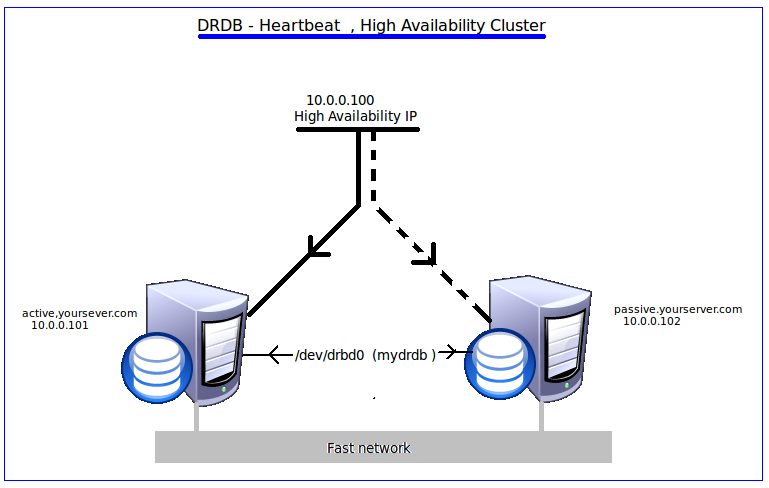
\includegraphics[scale=0.50]{drdb_hearbeat.png}
  \caption[High availability scheme]{High availability scheme}
  \label{fig:HAScheme}
\end{figure}

A reference to the bibliography~\cite{Fogel}.\\

This is a footnote\footnote{\url{http://www.apache.org/licenses/}}.

\begin{table}
  \centering
  \begin{tabular}{ | l | c | r | }
    \hline
    1 & 2 & 3 \\
    4 & 5 & 6 \\
    7 & 8 & 9 \\
    \hline
  \end{tabular}  
  \caption{This is a table}
  \label{table:tablename}
\end{table}

\section{Section}
\label{sec:section}

Reference to Table~\ref{table:tablename} 

	\subsection{Subseccion}
	\label{subsec:subsection}

This is another footnote\footnote{\url{http://www.fsf.org/}}.\\

Here are some items:

\begin{itemize}
	\item One
	\item Two
\end{itemize}

\section{Document Structure}
\label{sec:structure}

The way the dissertation is to be organised..


%=====================================
% PROBLEM STATEMENT 
%
\chapter{Problem statement}
\label{chap:problem}

Text..

\section{Justification / Motivation}
\label{sec:justification}

Text..

	\subsection{Subseccion}
	\label{subsec:subsection}

Text..

\section{Objetives}
\label{sec:objetives}

- General objetives\\
- Specific objetives

\section{Scope}
\label{sec:scope}

Text..


%=====================================
% PRECEDENTS / RELEATED TECHNOLOGIES / STATE OF THE ART
%
\chapter{Precedents / Releated technologies / State of the art}
\label{chap:precedents}

- High Availability solutions based in FLOSS


%=====================================
% METHODOLOGY
%
\chapter{Methodology}
\label{chap:methodology}

- Implemented technologies

%=====================================
% IMPLEMENTATION
%
\chapter{Implementation}
\label{chap:implementation}

\section{Technical specifications of implemented FLOSS tools}
\label{sec:specifications}

Text..

\section{Tets and validation}
\label{sec:tests}

Text..

\section{Other considerations}
\label{sec:considerations}

- Solution complements

%=====================================
% RESULTS AND DISCUSSION
%
\chapter{Results and discussion}
\label{chap:results}

Text..


%=====================================
% CONCLUSIONS
%
\chapter{Conclusions and future work}
\label{chap:conclusions}

Text..

%=====================================
% REFERENCES
%
\renewcommand{\bibname}{References}

\begin{thebibliography}{25}
  \bibliographystyle{alpha}

  \bibitem{Fogel} Fogel, Karl. \textit{Producing Open Source Software: How to Run a Successful Free Software Project}. O'Reilly, 2005.

  \bibitem{Raymond} Raymond, Eric. \textit{The Cathedral and the Bazaar}. O'Reilly, 1999.

\end{thebibliography}

%=====================================
% APPENDIX
%
\appendix
\chapter{Title of appendix 1}
\label{app:apendix1}


\end{document}